% LaTeX Template for Project Report, Version 2.0
% (Abstracted from a Major Project Report at CSED, NIT Calicut but can be
% modified easily to use for other reports also.)
%
% Released under Creative Commons Attribution license (CC-BY)
% Info: http://creativecommons.org/licenses/by/3.0/
%
% Created by: Kartik Singhal
% BTech CSE Batch of 2009-13
% NIT Calicut
% Contact Info: kartiksinghal@gmail.com
%
% It is advisable to learn the basics of LaTeX before using this template.
% A good resource to start with is http://en.wikibooks.org/wiki/LaTeX/
%
% All template fields are marked with a pair of angular brackets e.g. <title here>
% except for the ones defining citation names in ref.tex.
%
% Empty space after chapter/section/subsection titles can be used to insert text.
%
% Just compile this file using pdflatex after making all required changes.

\documentclass[12pt,a4paper]{report}
\usepackage[pdftex]{graphicx} %for embedding images
\usepackage{url} %for proper url entries
\usepackage[bookmarks, colorlinks=false, pdfborder={0 0 0}, pdftitle={<pdf title here>}, pdfauthor={<author's name here>}, pdfsubject={<subject here>}, pdfkeywords={<keywords here>}]{hyperref} %for creating links in the pdf version and other additional pdf attributes, no effect on the printed document
%\usepackage[final]{pdfpages} %for embedding another pdf, remove if not required

\begin{document}
\renewcommand\bibname{References} %Renames "Bibliography" to "References" on ref page

%include other pages
\begin{titlepage}

\begin{center}

\textup{\large {\sc Multi-core Programming} \\ \sc \small{Final Project Report}}\\[0.4in]

% Title
\Large \textsc {Implementation and Optimization of Image Template Matching in CUDA}\\[0.5in]

\vspace{0.1in}
       \small \emph{Submitted in partial fulfillment of\\
        the degree}
        \vspace{.2in}

       {\sc Bachelor of Science \\in\\ Software Engineering}\\[0.5in]

\vspace{0.3in}
% Submitted by
\normalsize Submitted by\\
\vspace{0.06in}
\textsc{\large Ali Gholami}

\vspace{.3in}
Under the guidance of\\
\vspace{0.06in}
\textsc{\large Prof. Mahmoud Momtazopur}

\vfill

% Bottom of the page

\includegraphics[width=0.25\textwidth]{nitc-logo}\\[0.1in]
\normalsize{Department of Computer Engineering and Information Technology}\\
\normalsize
\textsc{Amirkabir University of Technology}\\
\vspace{0.5cm}
Spring Semester 2018

\end{center}

\end{titlepage}

\vspace{2in}
\begin{abstract}

In most computer vision and image analysis problems, it is necessary to define a similarity measure between two or more different objects or images. Template matching is a classic and fundamental method used to score similarities between objects using certain mathematical algorithms\cite{abstract}. In this project, we'll propose two implementations of image template matching in CUDA. Our first method is based on the \textit{naive} version of the template matching and the second method is based on the \textit{Fast Fourier Transform} algorithm.

\end{abstract} 


\pagenumbering{roman} %numbering before main content starts
\tableofcontents
\listoffigures

\newpage
\pagenumbering{arabic} %reset numbering to normal for the main content

\chapter{Introduction}

In this section we'll take a brief look at the recent researches on \textit{Template Matching} task, its variants and the reliability of the models proposed in this task.
\section{Background and Recent Research}

\subsection{Feature Based Approach}
A featured-based approach is appropriate when both reference
and template images contain more correspondence
with respect to features and control points. In this case,
features include points, curves, or a surface model to perform
template matching. In this category, the final goal is to locate
the pair-wise connections between the target or so-called
reference and the template image using spatial relations
or features. In this approach, spatial relations, invariant
descriptors, pyramids, wavelets and relaxation methods play
an important role in extracting matching measures\cite{abstract}.

\subsection{Area Based Approach}
Area-based methods, which are usually known as correlation
methods or template matching, were developed for the
first time by Fonseca et al. [6] and are based on a combined
algorithm of feature detection and feature matching. This
method functions very well when the templates have no
strong features with an image, since they operate directly on
the pixel values. Matches are measured using the intensity
values of both image and template. The matching scores
are extracted by calculating squared differences in fixed
intensities, correction-based methods, optimization methods
and mutual information\cite{intro1}.

\subsection{Naive Template Matching}
Nave template matching is one of the basic methods of
extracting a given which is identical to the template from
the image target. In this approach, with or without scaling
(usually without scaling), the target image is scanned by the
template, and the similarity measures are calculated. Finally,
the positions with the strongest similarities are identified as
potential pattern positions\cite{abstract}. 

\subsection{Image Correlation Matching}
In this classic template matching method, the similarity
metric between the target and the template is measured.
Unlike the naive template matching algorithm, the target and the template might have different image intensities or
noise levels. However, those images must be aligned. The
similarity metric used in this approach is based on the
correlation between the target and the template\cite{intro2}.

\subsection{Sequential Similarity Detection Algorithms}
Sequential similarity detection algorithms (SSDAs) are
a more efficient alternative to correlation-based methods,
including matched filters for translational registration. The
measure of match is indirectly calculated based on an error
for corresponding pixels in f and g in the images under
comparison at any stage of the registration process\cite{intro3}.

\section{Motivation}
There are dozen optimized implementation of \textit{Template Matching} techniques, but the main motivation for me to do so, was the ability to model and code a real-life problem from scratch. I've also improved my CUDA and C++ programming skills with this project. Also, there are multiple math concepts covered in the \textit{Fast Fourier Transform} section which understanding them can bring an enhanced point of view in image and signal processing tasks. %literature survey included in this
\chapter{Problem Definition}

The emerging need of image processing techniques in everyday life is inevitable. There have been lots of image processing algorithms proposed to increase the overall availability of tools in image understanding and using these tools to improve the human life. \textit{Template Matching} is a task that its applications are obvious in everyday life. Computer vision tasks such as \textit{object detection}, \textit{object recognition} and other tasks based on these two main questions; Is there a certain object in the image? And if yes, where is it in the image?, can be classified as subproblems of \textit{template matching} task. This task can be extended to counting the number of occurrences of an object in a given image. Given a main image and a template image, we want to find occurrences of the template image in main image. This problem can be solved in many ways. In the next chapter, we'll analyze the procedure of \textit{naive} template matching to solve this problem. In further chapters, we'll provide the procedure of using \textit{Fast Fourier Transform} to convert the images into frequency domain. We'll show that finding the maximum value of the result of the convolution of two images is where the template has occurred in main image.

\section{Naive Template Matching}
The main task of naive template matching was clearly explained in the previous section. There are various similarity measures in naive template matching. The one we use here is \textit{SAD} or \textit{Sum of Absolute Deviations} which is formally described further. Let $f$ and $t$ be the main image and the template image respectively and $(x, y)$ represent the column and the row of each image. The \textit{Sum of Absolute Deviations} error metric for two images can be written as:
\begin{equation}
	SAD = \sum_{x, y}^{}f(x, y) - t(x - u, y - v)
\end{equation}

Note that there is also a more precise error metric called \textit{Sum of Squared Errors} which is represented as:
\begin{equation}
		SSD = \sum_{x, y}^{}[f(x, y) - t(x - u, y - v)]^2
\end{equation}
In this project, we'll use the first error metric because of the processing power limits.

\section{FFT-Based Template Matching}
\subsection{One-Dimensional Discrete Fourier Transform}
The Fourier transform of a discrete function of one variable, $f(x)$, $x = 0, 1, 2, ..., M-1$, is given by the equation
\begin{equation}
	F(u) = \frac{1}{M}\sum_{x = 0}^{M - 1} f(x) e^{-j2\pi ux/M} \ \ \ \ u = 0, 1, 2, ..., M-1
\end{equation}
Similarly, given $F(u)$, we can obtain the original function back using the inverse DFT:
\begin{equation}
	f(x) = \sum_{u = 0}^{M -1}F(u)e^{j2\pi ux /M} \ \ \ \ x = 0, 1, 2, ..., M - 1
\end{equation}
\subsection{Two-Dimensional Discrete Fourier Transform}
Extension of the one-dimensional discrete Fourier transform and its inverse to two dimensions is straightforward. The discrete Fourier transform of a function (image) $f(x, y)$ of size $M * N$ is given by the equation
\begin{equation}
	F(u, v) = \frac{1}{MN}\sum_{x = 0}^{M - 1}\sum_{y = 0}^{N - 1}f(x, y)e^{-j2\pi(ux/M + ry/N)}
\end{equation}
As in the 1-D case, this expression must be computed for values of $u = 0, 1, 2, ..., M -1 $, and also for $v = 1, 2, ..., N -1 $. Similarly, given $F(u, v)$, we obtain $f(x, y)$ via the inverse Fourier transform, given by the expression
\begin{equation}
	f(x, y) = \sum_{u = 0}^{M -1}\sum_{r = 0}^{N - 1} F(u, v)e^{j2\pi (ux/M + ry/N)}
\end{equation}

\subsection{Convolution and Correlation Theorems}
The discrete convolution of two functions $f(x, y)$ and $h(x, y)$ of size $ M * N$ is denoted by $f(x, y) \star h(x, y)$ and is defined by the expression
\begin{equation}
	f(x, y) \star h(x, y) = \frac{1}{MN}\sum_{m = 0}^{M - 1}\sum_{n = 0}^{N - 1}f(m, n)h(x - m, y-m)
\end{equation}
we also know that the convolution theorem consists of the following relationships between the two functions and their Fourier transforms:
\begin{equation}
	f(x, y) \star h(x, y) \leftrightarrow F(u, v)H(u, v)
\end{equation}
and 
\begin{equation}
	f(x, y)h(x, y) \leftrightarrow F(u, v) \star H(u, v)
\end{equation}
The correlation of two functions $f(x, y)$ and $h(x, y)$ is defined as
\begin{equation}
	f(x, y)\circ h(x, y) = \frac{1}{MN} \sum_{m = 0}^{M - 1}\sum_{n = 0}^{N - 1}f^*(m, n)h(x + m, y + n)
\end{equation}
where $f^*$ denotes the complex conjugate of $f$. Convolution is the tie between filtering in the spatial and frequency domains. The principal use of correlation is for matching. In matching, $f(x, y)$ is an image containing objects or regions. If we want to determine whether $f$ contains a particular object or region in which we are interested, we let $h(x, y)$ be that object or region (we call this image a template). Then, if there is a match, the correlation of two functions will be maximum  at the location where $h$ finds a correspondence in $f$. An example of this phenomenon is provided in figure 2.1.
\begin{figure}[!h]\centering
	
\includegraphics[width=0.8\textwidth]{figure_2_1.PNG}
	\caption{Illustration of image padding and correlation. The highest value of the correlation function occurs at the point where template is exactly on top of the \textit{T} in the image.}
	\label{pl1}
\end{figure}

\section{Fast Fourier Transform}
One of the main reasons that the DFT has became an essential tool in signal processing was the development of the fast Fourier transform. Computing the 1-D Fourier transform of $M$ points requires on the order of $M^2$ multiplication/addition operations. The FFT accomplishes the same task on the order of $M \log_2 M $ operations. If, for example $M = 1024$, the brute-force method will require approximately $10^6$ operations. While the FFT will require approximately $10^4$ operations. This is a computational advantage of 100 to 1. The decrease in computational complexity significantly impacts the time needed for processing the images. The FFT algorithm is based on the so-called \textit{successive doubling method}. Let's define the equation
\begin{equation}
	F(u) = \frac{1}{M} \sum_{x = 0}^{M - 1}f(x)W_M^{ux}
\end{equation}
where 
\begin{equation}
	W_M = e^{-j2\pi / M}
\end{equation}
and $M$ is assumed to be of the form
\begin{equation}
	M = 2^n
\end{equation}
with $n$ being a positive integer. Hence, $M$ can be expressed as 
\begin{equation}
	M = 2K
\end{equation}
Substitution of (2.14) into (2.11) yields
\begin{equation}
	F(u) = \frac{1}{2}[\frac{1}{K}\sum_{x = 0}^{K - 1} f(2x)W^{u(2x)}_{2K} + \frac{1}{K}\sum_{x = 0}^{K - 1}f(2x + 1)W_{2k}^{u(2x + 1)}]
\end{equation}
The number of multiplications and additions required to implement FFT:
\begin{equation}
	m(n) = 2m(n - 1) + 2^{n - 1} \ \ \  n \geq 1 = \frac{1}{2} M \log_2 M
\end{equation}
and
\begin{equation}
	a(n) = 2a(n - 1) + 2^n  \ \ \ n \geq 1 = M \log_2 M
\end{equation} %objective changed to problem definition
\chapter{Implementation and Performance Analysis}

\section{Analysis of Naive Template Matching}
In this section, we'll analyze the implementation and the performance of the \textit{Naive Template Matching} algorithm. First of all, let's consider the serial implementation case. 

\subsection{Bitmap Images}
For this project, we've used the \textit{bitmap} image library by \textit{Arash Partow} which is accessible \href{https://github.com/ArashPartow/bitmap}{here}.

\subsection{Serial Implementation of NTM}
The serial implementation of this algorithm consists of 2 main loops to iterate over image pixels. There is also a need for each pixel we are iterating through, to calculate the \textit{Sum of Absolute Deviations} which is the similarity measure between the main image pixels and the template image. Please refer to the \textit{Naive Template Matching} algorithm to see the code. Since the task is mainly focused on counting the number of occurance inside the main images, we can obtain this by finding the minimum value of \textit{SAD} while iterating through the main image pixels and counting the number of occurrences of the found minimum inside the main image matrix.

\subsection{Timing the Serial NTM}
We can obtain the elapsed time for the serial iteration using the \textit{chrono} library. The code for this section is provided here. Please refer to the serial implementation code for the details. 

\subsection{CUDA Implementation of NTM}
In this section we'll walk through the kernel codes provided in the \textit{kernel.cu}.
\subsubsection{Compute Sad Array Kernel}
The image data is being stored in an 1-D array. Thus, the best choice for CUDA kernel launch parameters would be to set grid dimensions as $(image\_width/block\_size\_x, image\_height/block\_size\_y, 1)$. The main purpose of this choice is not the way we have stored the data, it actually depends on the input data. Since we are dealing with images it is more suitable to have 2-D blocks of threads. Further explanations focus on the kernel implementation. Initially, each thread finds its own global 2-D identification as rows and columns. Then, each thread virtually sees a kernel (template) around it self. This is the core of the parallelization section. All threads can see all of the iterations in one place. We then compute the SAD of each pixel and load it inside an SAD array. The next section describes the reason to do so.

\subsubsection{Find Minimum in Array Kernel}
We can obtain the best possible match by finding the minimum SAD in SAD array. We'll do so using shared memory to speed up the process. Each thread helps loading the data inside a block into the shared memory of that block. We then use \textit{fminf} to find the minimum inside each block. Since we are using the shared memory, we need to do a \textit{reduction} to find the minimum across different blocks. We can obtain this reduction task defining a \textit{mutex} to control the global memory write by first thread of each block.

\subsubsection{Find Number of Occurrences}
Since the main task is to find the number of occurrences of template image in main image, we should count the number of occurrences of minimum SAD in the SAD array. To speed up the process we've used shared memory again. The intuition of using shared memory is exactly the same as the previous section.

\subsection{Launch Parameters on Test Cases}
The test has been done on three different sizes of images. One of the medium sized images is a \textit{bitmap} image with dimensionality of $1112 * 1500$. The template image is a $116*116$ image in this case. Considering a block size of 1024 on a \textit{Nvidia 850m GTX} (compute capability of 5), the launch parameters are provided below:
\begin{figure}[!h]\centering
	
\includegraphics[width=0.6\textwidth]{grid_block.PNG}
	\label{pl1}
\end{figure}

\subsection{Occupancy Analysis}
Before getting into the details, it is important to mention that maximum number of active warps in theory is 64. \textit{Nsight} profiler provides great details on the number of active warps per SM. In this case, there are 63.83 active warps on the first kernel (Compute Sad Array Kernel). The occupancy can obtained by dividing the number of active warps to the number of maximum warps available:
\begin{equation}
	 occupancy = \frac{63.83}{64} = 99.74 \%
\end{equation}
\begin{figure}[!h]\centering
	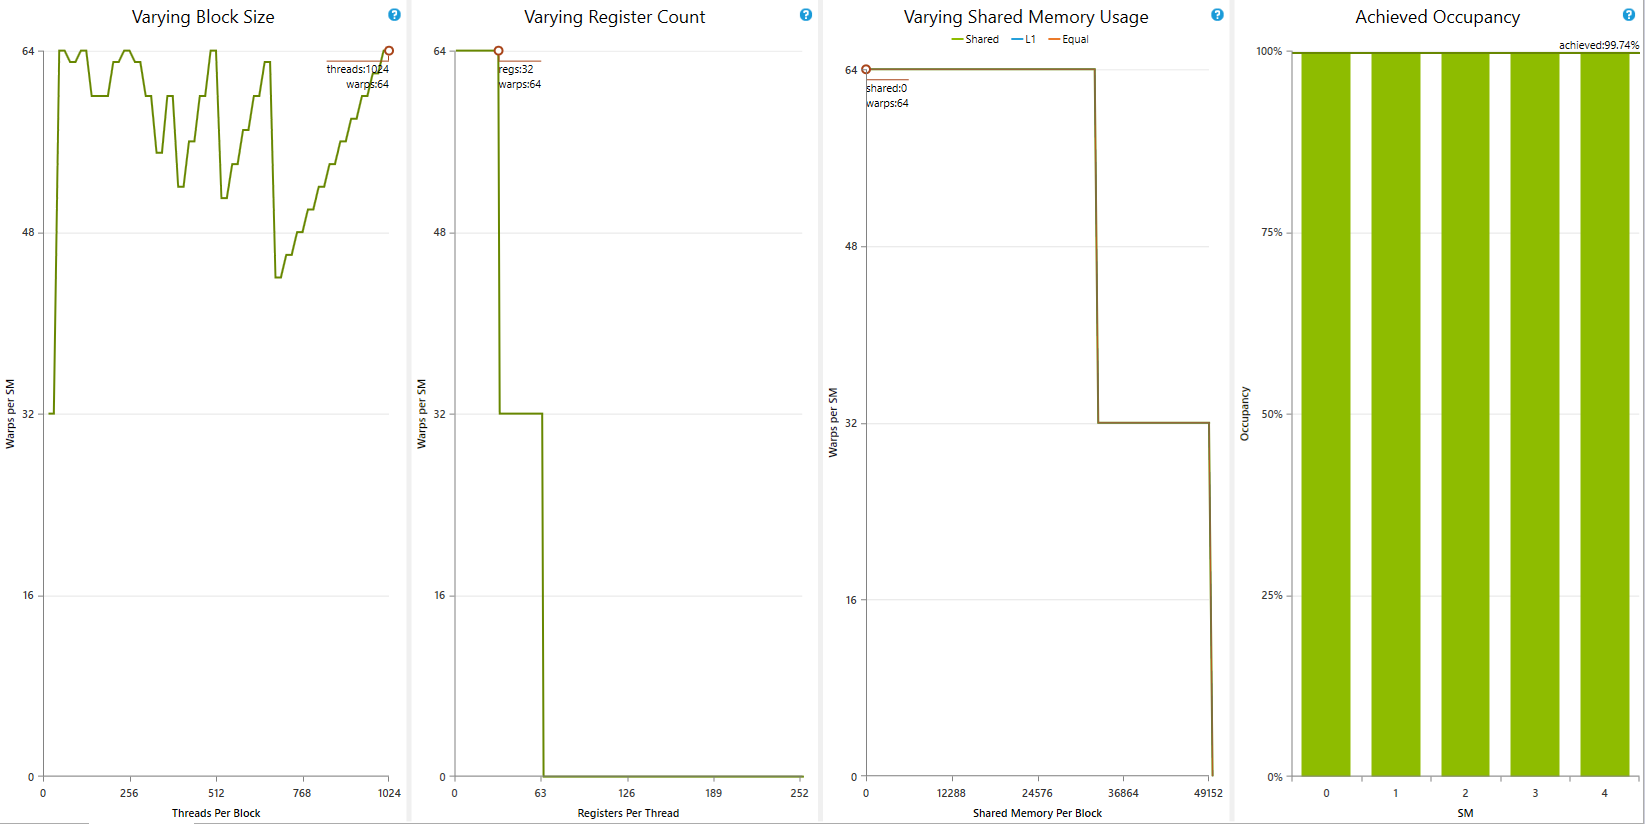
\includegraphics[width=0.99\textwidth]{occupancy_analysis.PNG}
	\caption{Illustration of varying the size of blocks, registers and shared memory on the achieved occupancy.}
	\label{pl1}
\end{figure}

According to figure 3.1, varying the number of threads per block might yield the same result in other scenarios. The circled point shows the current number of threads per block and the current upper limit of active warps. Note that the number of active warps is not the number of warps per block (that is threads per block divided by warp size, rounded up). If the chart's line goes higher than the circle, changing the block size could increase occupancy without changing the other factors.  Also, increasing the number of variables (registers per block) will drastically decrease the occupancy of the first kernel.

\subsection{SM Activity Analysis}
\begin{figure}[!h]\centering
	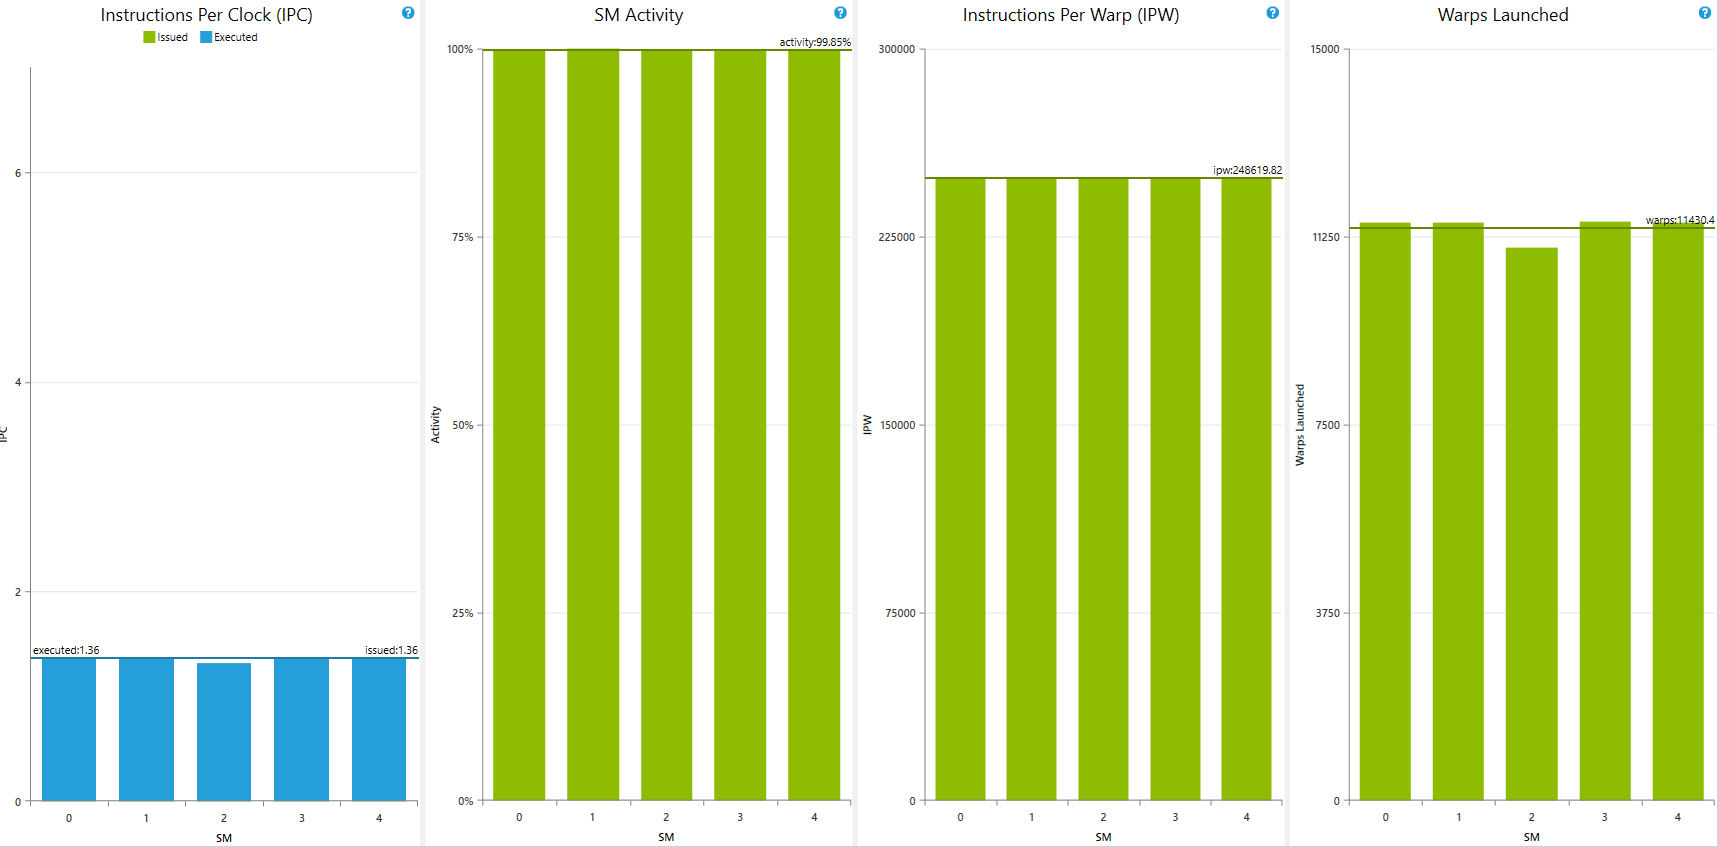
\includegraphics[width=0.99\textwidth]{sm_activity.PNG}
	\caption{Issue efficiency and SM activity charts for the first (bottleneck) kernel.}
	\label{pl1}
\end{figure}
The IPC chart demonstrates the achieved instructions throughputs per SM for both, issued instructions and executed instructions. The theoretical maximum peak IPC is a device limit and defined by the compute capabilities of the target device.

\subsubsection{Issued IPC}
The average number of issued instructions per cycle accounting for every iteration of instruction replays. Optimal if as close as possible to the Executed IPC. As described in the background section of this document, some assembly instructions require to be multi-issued. Hence, the instruction mix affects the definition of the optimal target for this metric. In this case, the issued IPC throughput is minimum since there weren't any multi issue instructions in the first kernel.

\subsubsection{Executed IPC}
The average number of executed instructions per cycle. Each warp scheduler of a multiprocessor can execute instructions independently, a target goal of executing one instruction per cycle means executing on average with an IPC equal to the number of warp schedulers per SM. The maximum achievable target IPC for a kernel is dependent on the mixture of instructions executed. 

\subsubsection{SM Activity Chart}
The second chart provides information on the activity of each SM during the kernel launch. A multiprocessor is considered to be active if at least one warp is currently assigned for execution. An SM can be inactive - even though the kernel grid is not yet completed - due to high workload imbalances. Such uneven balancing between the SMs can be caused by a few factors: Different execution times for the kernel blocks, variations between the number of scheduled blocks per SM, or a combination of the two. In this case, non of the above has occurred and the activity result is almost 100\%.

\subsubsection{IPW Chart}
One of the most common patterns for varying IPWs is conditionally executed code blocks. IPW can be useful while having variations in SM activity chart which in this case, non of these have occurred.

\subsection{Speedup Analysis}
In this section, we'll analyze the possible theoretical speedup. For this purpose, we'll calculate the serial computation time for the \textit{collection} and \textit{collection\_coin} images as described above. This table describes the average speedup of parallel naive template matching algorithm compared to serial implementation. As can be seen in the figure 3.3, the speedup obtained on GPU is dedicated to many different parameters. In order to calculate the theoretical speedup a direct use of \textit{Amdahl's law} doesn't fit in this problem. One might say that the number of cores in this case is \textit{N} (Same as the number of threads), but GPU does not have as many physical cores as the number of threads that can be launched. Additionally, significant portion of kernel time is begin spent just waiting for the data to be \textit{read/written} from/to global memory. Also, the frequency and operational power of CPU cores is higher than GPU cores. In this section, we'll use a modified version of the Amdahl's law \cite{amdahl}:
\begin{equation}
	S = \frac{1}{(1 - p) + (k * p / N)} \ \ \ \ \  \ k = freq(CPU) / freq(GPU)
\end{equation}
The core frequency of my Intel 4710HQ processor is 3490 MHz. The core frequency of each GPU core is 902 MHz. These information are extracted using beloved \textit{CPU-Z} and \textit{GPU-Z} programs. Replacing these information into 3.2 yields
\begin{equation}
	S = \frac{1}{(1 - p) + 3.86 * p / N}
\end{equation}
since the size of input is constant in this law, we'll assume that 3.3 is correct for the third experiment. Let's suppose that $\frac{1}{4}$ of the main program is parallelized, thus $p = \frac{1}{4}$ and the number of threads to run is 1828864 (1786 blocks of 1024). Theoretical speedup will be
\begin{equation}
	S = \frac{1}{(\frac{3}{4}) + 3.86 * \frac{\frac{1}{4}}{1828864}} = 1.33
\end{equation}
\begin{figure}[!h]\centering
	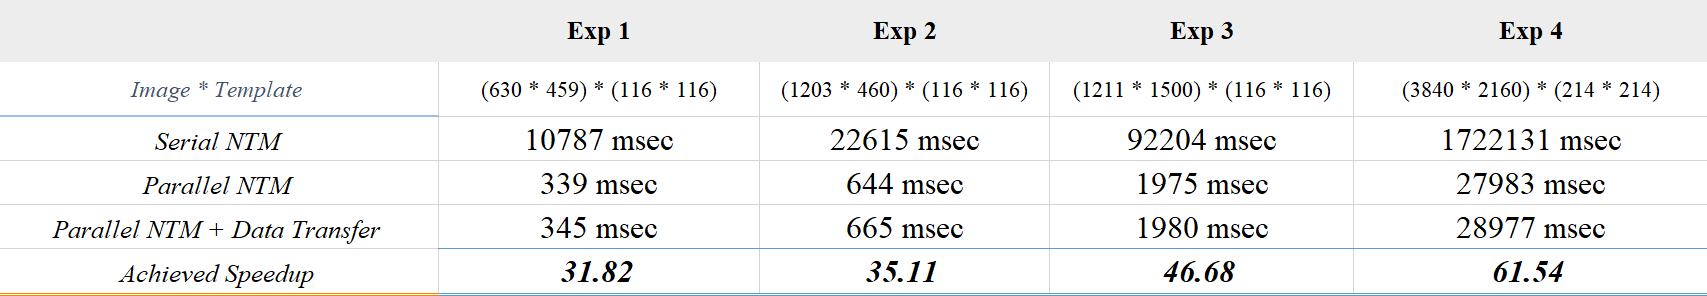
\includegraphics[width=0.99\textwidth]{speedup.PNG}
	\caption{Computation and data transfer time for naive serial and parallel implementation.}
	\label{pl1}
\end{figure}

\subsection{Performance Analysis}
In this section, we'll analyze the performance of the \textit{Compute Sad Array Kernel}. Firstly, lets find the arithmetic intensity of this kernel. Arithmetic intensity $I$, also called \textit{operational intensity}, is the ratio of \textit{arithmetic operations} or \textit{work} ($W$), to the \textit{memory traffic} ($Q$) \cite{roofline}:
\begin{equation}
	I = \frac{W}{Q}
\end{equation}
and denotes the number of operations per byte of memory traffic. When the work is represented as \textit{FLOPS}, the arithmetic intensity will be \textit{FLOPS/Byte}. According to the \textit{Naive Roofline Model}, the \textit{attainable performance} is bound either by the \textit{peak performance} or \textit{memory bandwidth * arithmetic intensity}. In this case, the operational intensity can be obtained by following the memory access patterns and the work being done in the main kernel:
\begin{figure}[!h]\centering
	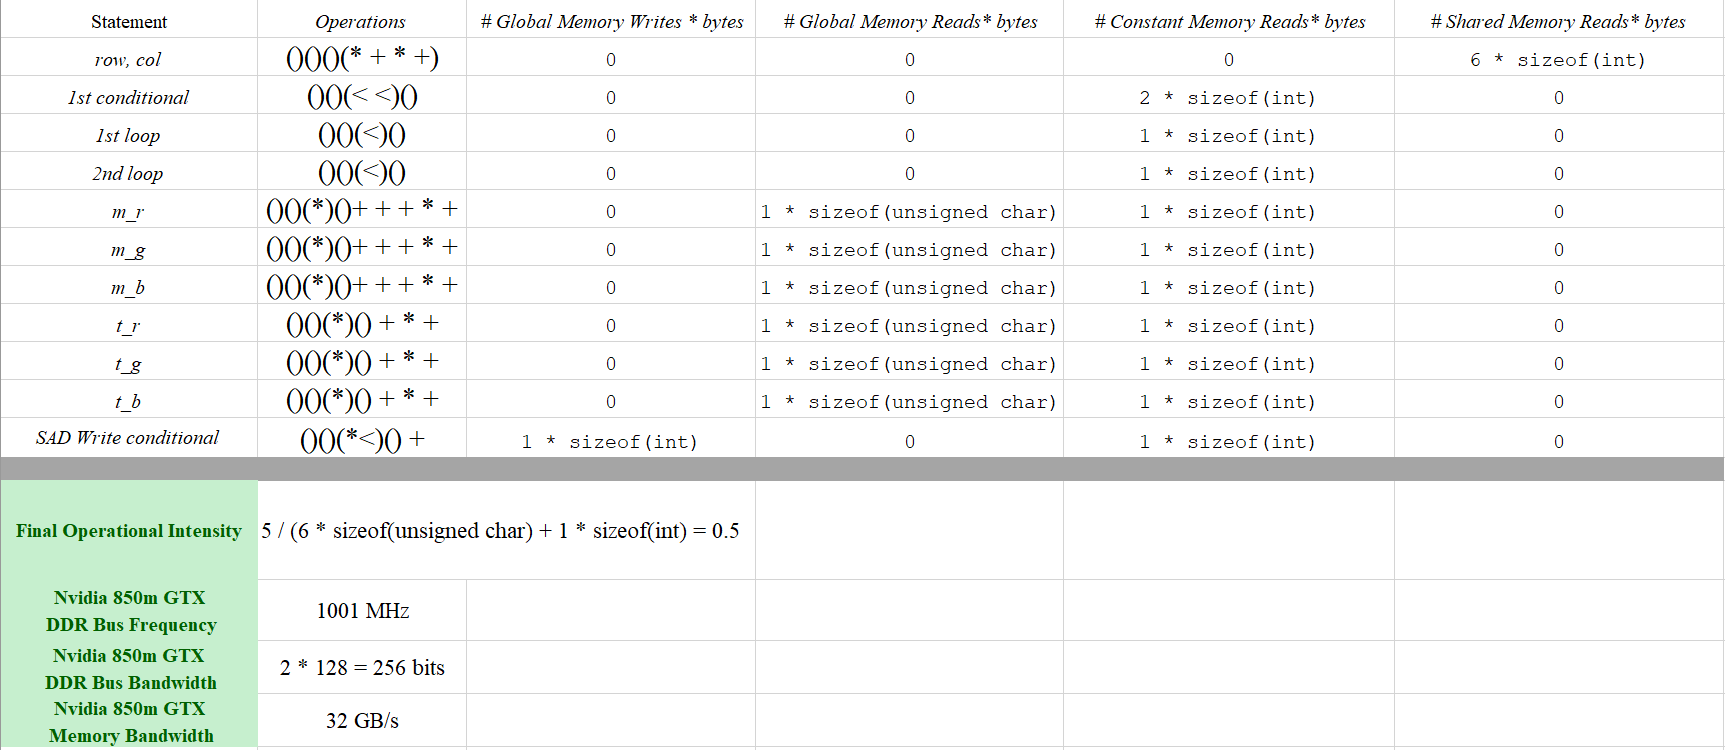
\includegraphics[width=1\textwidth]{intensity.PNG}
	\caption{Calculation of first kernel operational intensity and GPU memory bandwidth.}
	\label{pl1}
\end{figure}
It is given that the \textit{single precision} processing power of a \textit{Nvidia 850m GTX} is 1155 GFLOPS \cite{techpower}. Given these results, the kernel is actually memory bound since $0.5 < 1155 / 32 = 36$. The kernel arithmetic intensity should be at least 36 to be considered a compute bound kernel.

\section{Implementation of FFT Based Template Matching}
In this section, we delve into the details of \textit{FFT} based template matching using \textit{cufft} library from \textit{Nvidia}. Note that this implementation is still in progress and there are multiple serial loops conducted in preprocessing step which slows down the process compared to the \textit{naive template matching} procedure.
As mentioned before, the overall procedure is to convert the spatial domain of input images to the frequency domain. In the frequency domain, we can apply a correlation based operation. This operation yields a signal of the same size as main image size. We then apply an inverse Fourier transform to turn the results back to the spatial domain. We then find the maximum of that signal and the number of occurrences of that maximum value in that signal. The procedure is well defined below\cite{gonzalez}:
\begin{equation}
	c = real(IFFT_{2D} (FFT_{2D}(main\_image) .* FFT_{2D}(template\_image)))
\end{equation}	
according to 3.6, $c$ contains a list of values which we are desired to find the maximum of it (for maximum similarity). To obtain this in CUDA, we've used multiple functions which are described further. Note that \textit{*} symbol shows the complex conjugate of the second signal.

\subsection{Real to Complex Conversion}
For this part, we have not focused on the performance. We use simple \textit{for} loops to convert the image data matrix to the proper format of \textit{cufft} library which is called \textit{cufftComplex}. \textit{cufftComplex} is a simple typedef of \textit{float} type in C.

\subsection{Padding Data}
Before performing a \textit{2-D Forward Fourier Transform} we are urged to perform a data padding on template signal to make it the same size as the main signal. Figure 2.1 illustrates this phenomenon pretty well. The duty of data padding is simple. Allocate new memory with a new size. Copy signals into their corresponding location in new allocated memory and set other places to 0.

\subsection{2-D FFT Planning}
\textit{cufft} library uses the concept of \textit{plan} to provide the baseline setup for the main APIs provided in the library. A plan can initiate a 1-D, 2-D or 3-D data processing API from \textit{cufft} library. In this implementation, we need a setup for a 2 dimensional Fourier transform, thus we use \textit{cufftPlan2d} to prepare the library for the main transformations.

\subsection{Forward FFT Launch}
In order to launch a forward \textit{complex to complex} Fourier transform using \textit{cufft}, we'll use \textit{cufftExecC2C}. The constant \textit{CUFFT\_FORWARD} shows the direction of the Fourier transform which is \textit{Forward} in this case.

\subsection{Complex Conjugate Kernel}
This kernel implements the conjugation procedure. The implementation is pretty straightforward. Each thread multiples the corresponding signal point's complex part to -1 and loads it back to the input signal.

\subsection{Complex Point-wise Kernel}
This kernel provides a point to point multiplication manner for each of the points in main and template input signals. It uses another kernel called \textit{ComplexMul} to perform a \textit{complex multiplication}. It then scales the result using \textit{ComplexScale}. Scaling or normalization is mainly done by dividing the signal values to the size of the signal.

\subsection{Inverse FFT Launch}
Finally, we'll perform an inverse Fourier transform on the result of the \textit{Complex Point-wise Kernel}. The resulting signal is in the spatial domain.

\subsection{Maximum Value and Number of Occurrences}
To find the number of occurrences, we \textit{serially} iterate over the resulting signal of the previous section. Note that these steps are not \textit{100\%} efficient and are still in improvement.
\chapter{Future Work}
We admit the possible drawbacks and inefficiencies existing in this project, thus we have the following key improvement to-do list:
\begin{itemize}
	\item Reorganization of the project structure, header files and .c files.
	\item Reorganization of the project source code for a C unified implementation.
	\item Usage shared memory techniques to improve the performance of the \textit{NTM} implementation.
	\item Usage of highly-optimized image libraries such as \textit{OpenCV} for \textit{image rotation}, \textit{image matrix extraction} and general \textit{bitmap processing}.
	\item Implementation of CUDA kernels for real-to-complex signal conversions.
	\item Implementation of CUDA kernel to find the number of occurrences of template signal in main signal in \textit{Fourier} based template matching.
\end{itemize}
\chapter{Conclusion}

<Conclusion here>

\cleardoublepage
%\pagebreak
\phantomsection
\addcontentsline{toc}{chapter}{Acknowledgements}
\chapter*{Acknowledgments}
\vspace{1.0in}
<Acknowledgements here>
\\
\\
\\ 
\\
<Name here> \\ 
\\
<Month and Year here>\\
{National Institute of Technology Calicut}\\
\newpage

\cleardoublepage
%\pagebreak
\phantomsection
\addcontentsline{toc}{chapter}{References}
\begin{thebibliography}{99}

\bibitem{abstract}Hashemi, Nazanin Sadat, et al. "Template Matching Advances and Applications in Image Analysis." arXiv preprint arXiv:1610.07231 (2016).


\bibitem{intro1}Mahalakshmi, T., R. Muthaiah, and P. Swaminathan. "An overview of template matching technique in image processing." Research Journal of Applied Sciences, Engineering and Technology 4.24 (2012): 5469-5473.

\bibitem{intro2}Perveen, Nazil, Darshan Kumar, and Ishan Bhardwaj. "An overview on template matching methodologies and its applications." IJRCCT 2.10 (2013): 988-995.

\bibitem{intro3}Cox, Greg S. "Template matching and measures of match in image processing." University of Cape Town, South Africa (1995).

\bibitem{amdahl}Andrey Alekseenko (https://stackoverflow.com/users/929437/aland), Amdahl's law and GPU, URL (version: 2018-07-13): https://stackoverflow.com/q/12398929.

\end{thebibliography}


\end{document}
